\let\negmedspace\undefined
\let\negthickspace\undefined
\documentclass[journal,12pt,onecolumn]{IEEEtran}
\usepackage{cite}
\usepackage{amsmath,amssymb,amsfonts,amsthm}
\usepackage{algorithmic}
\usepackage{graphicx}
\graphicspath{{./figs/}}
\usepackage{textcomp}
\usepackage{xcolor}
\usepackage{txfonts}
\usepackage{listings}
\usepackage{enumitem}
\usepackage{mathtools}
\usepackage{gensymb}
\usepackage{comment}
\usepackage{caption}
\usepackage[breaklinks=true]{hyperref}
\usepackage{tkz-euclide} 
\usepackage{listings}
\usepackage{gvv}                                        
%\def\inputGnumericTable{}                                 
\usepackage[latin1]{inputenc}     
\usepackage{xparse}
\usepackage{color}                                            
\usepackage{array}                                            
\usepackage{longtable}                                       
\usepackage{calc}                                             
\usepackage{multirow}
\usepackage{multicol}
\usepackage{hhline}                                           
\usepackage{ifthen}                                           
\usepackage{lscape}
\usepackage{tabularx}
\usepackage{array}
\usepackage{float}
%\newtheorem{theorem}{Theorem}[section]
%\newtheorem{theorem}{Theorem}[section]
%\newtheorem{problem}{Problem}
%\newtheorem{proposition}{Proposition}[section]
%\newtheorem{lemma}{Lemma}[section]
%\newtheorem{corollary}[theorem]{Corollary}
%\newtheorem{example}{Example}[section]
%\newtheorem{definition}[problem]{Definition}

\begin{document}

%\textbf{\Large 1.6.16} \\
%\textbf{\large AI25BTECH11001 - Abhisek Mohapatra} \\
\title{1.6.16}
\author{AI25BTECH11001 - ABHISEK MOHAPATRA}
% \maketitle
% \newpage
% \bigskip
%\begin{document}
{\let\newpage\relax\maketitle}
%\renewcommand{\thefigure}{\theenumi}
%\renewcommand{\thetable}{\theenumi}
% \newpage
% \bigskip
		\textbf{Question}:

		\noindent Find the values of $k$ if the points $\vec{A}(k +1,2k)$, $\vec{B}(3k, 2k +3)$ and $\vec{C}(5k-1,5k)$ are collinear.

		\textbf{Solution:} From the given information,


		\begin{align}
			\vec{A} = \myvec{k+1\\2k},\vec{B} = \myvec{3k\\2k+3},\vec{C} = \myvec{5k-1\\5k} 
		\end{align}
		To check if the points are collinear, we can use 
		\begin{align}
			rank\myvec{\vec{B}-\vec{A} & \vec{C}-\vec{A}} = 1	
		\end{align}
		So,
		\begin{align}
			\myvec{\vec{B}-\vec{A} & \vec{C}-\vec{A}}^T = \myvec{2k-1 & 3 \\ 4k-2 & 3k}	
			\\
			\xleftrightarrow[]{R_2 = R_2 - 2R_1} 
			\myvec{2k-1 & 3 \\ 0 & 3k-6} 
		\end{align}
		The rank of the matrix will be 1 when 
		\begin{align}
		3k-6 = 0
		\end{align}
		\begin{align}
		\Rightarrow k = 2
		\end{align}
		Graph:
\begin{figure}[H]
	\centering
	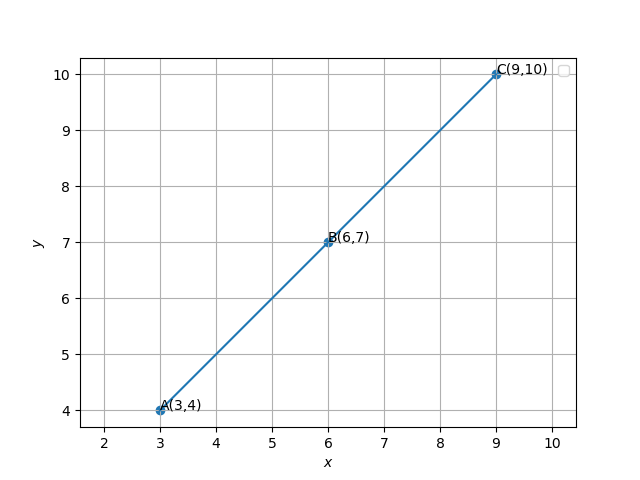
\includegraphics[scale=0.5]{img}
	\caption*{}
	\label{img}
\end{figure}


		Therefore, k = 2.
\end{document}


